\section{Resultados obtidos}
\label{sec:results}

\subsection{Modelo neutro}
Se não formos nem pessimistas nem otimistas, isto é, usando todos os valores apresentados na secção \label{sec:model} sem qualquer alteração, verifica-se que o \textit{Signal} possui o crescimento apresentado na figura \ref{model:base_signal_model}. Como é percetível da análise do terceiro gráfico da figura, temos um crescimento do valor da relação entre o número de utilizadores mensais e o número de \textit{downloads} lento, mas existente, sendo que ao final de 120 meses alcança um valor de 0.282792 (o valor no primeiro mês foi de 0.241579). Já o número de utilizadores ativos mensalmente teve uma subida linear, alcançando um valor de apróximadamente 28 milhões utilizadores ao final de 10 anos. Quanto ao número de \textit{downloads}, este teve um crescimento linear, aumentando de à volta de 20 milhões no inicio da simulação para aproximadamente 98 milhões de \textit{downloads}.

\begin{figure}[H]
   \begin{center}
       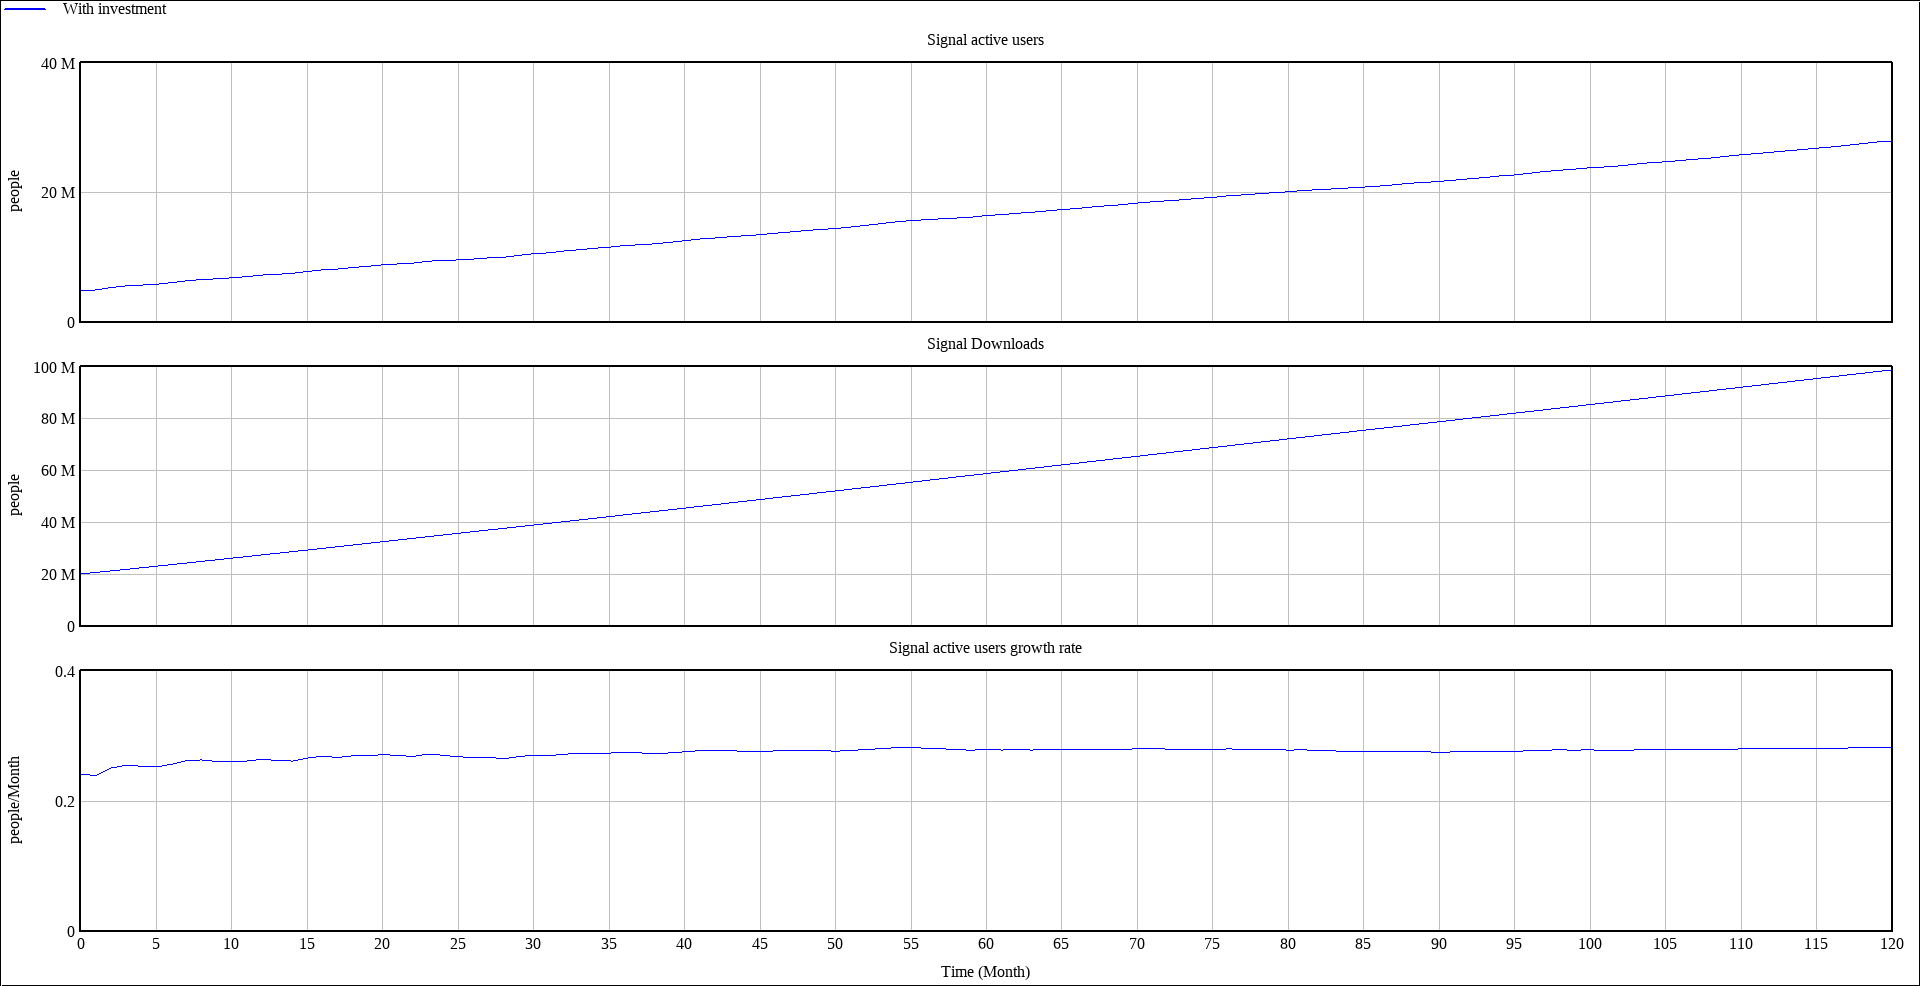
\includegraphics[width=17cm]{img/neutral_model_signal.png}
       \caption{Resultados do crescimento do número de utilizadores ativos, do número de \textit{downloads} e do valor da relação entre o número de \textit{downloads} e o número de utilizadores ativos do \textit{Signal}, obtidos numa execução neutra.}
       \label{model:base_signal_model}
   \end{center}
\end{figure}

Apesar do grande crescimento obtido, quando comparado com os dois serviços concorrentes, o número de utilizadores ativos é ainda muito inferior, como é possível verificar no gráfico da figura \ref{model:base_all_model}.

\begin{figure}[H]
   \begin{center}
       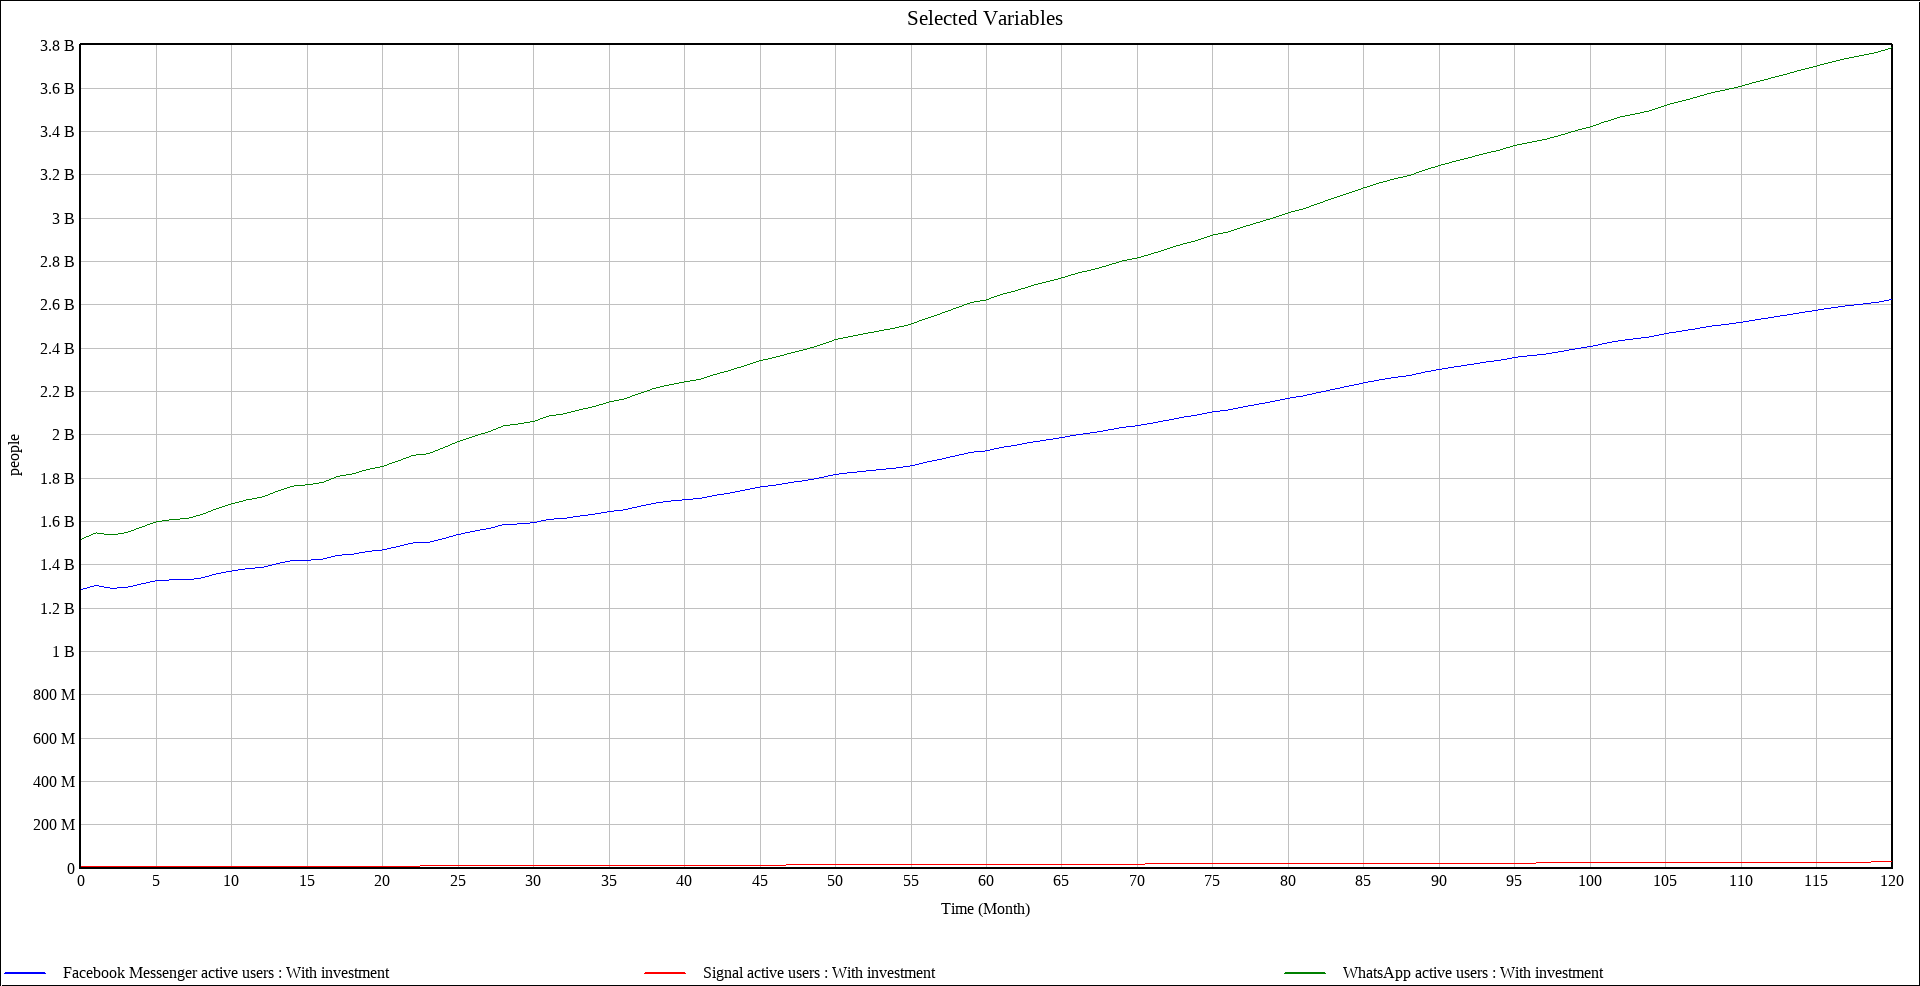
\includegraphics[width=17cm]{img/neutral_model_all.png}
       \caption{Resultados do crescimento do número de utilizadores ativos dos três serviços estudados, obtidos numa execução neutra.}
       \label{model:base_all_model}
   \end{center}
\end{figure}

Contudo, ao contrário do \textit{Signal}, as duas aplicações concorrentes tiveram uma descida ligeira ao longo do tempo no número médio de \textit{downloads} mensais, como é possível verificar na figura \ref{model:base_others_model}.

\begin{figure}[H]
   \begin{center}
       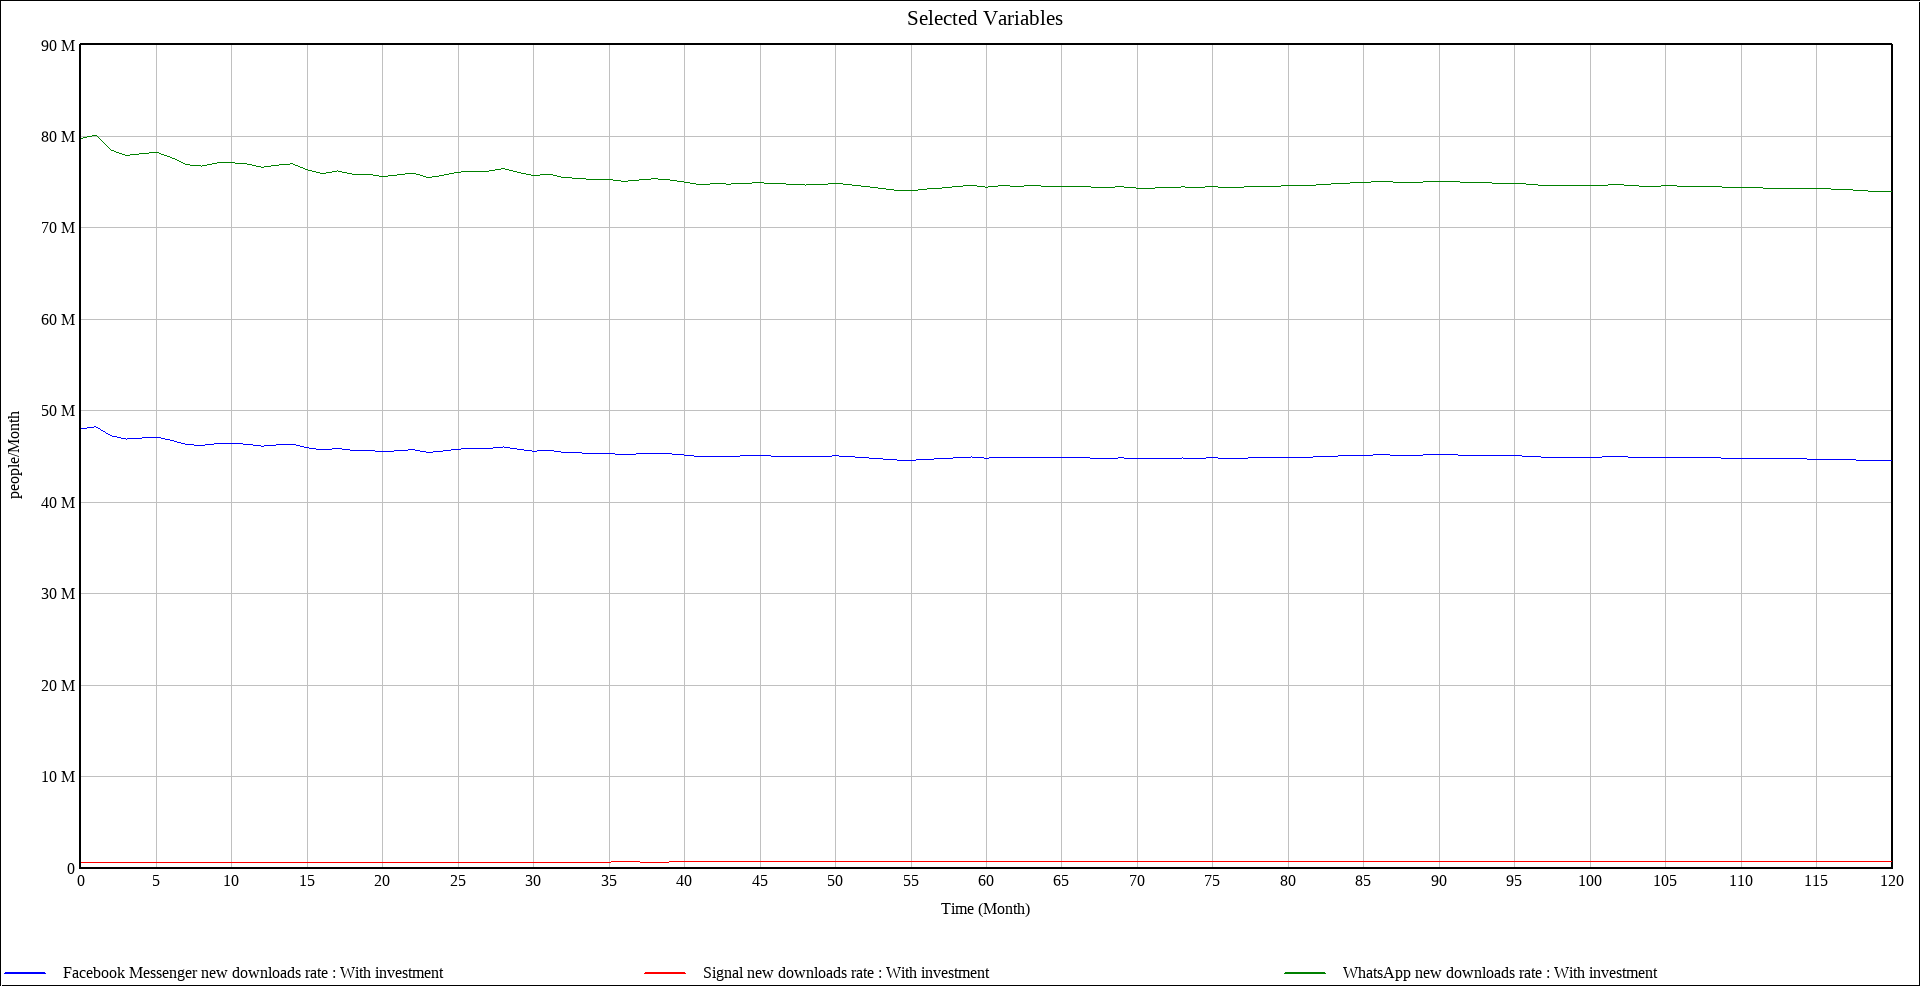
\includegraphics[width=17cm]{img/neutral_model_others_download_rate.png}
       \caption{Resultados do crescimento do número médio de \textit{downloads} mensais das aplicações concorrentes.}
       \label{model:base_others_model}
   \end{center}
\end{figure}


\subsection{Modelo pessimista}

O modelo apresentado anteriormente tem em conta que ao longo do tempo haverão investimentos de acordo com uma probabilidade hipotética. Contudo, esta probabilidade pode-se verificar muito inferior, podendo mesmo nunca chegar a haver novos investimentos. Para além disso, foi tida em conta que as aplicações concorrentes tinham um valor relativamente baixo de gastos mensais o que, dada a dimensão da empresa a que pertencem, pode não se verificar uma realidade. Desta forma, o modelo foi executado novamente, com as seguintes alterações:

\begin{itemize}
   \item Probabilidade de investimento - passou a ser $\frac{1}{100}$ ao invés de $\frac{1}{48}$.
   \item Valor máximo do investimento - passou a ser de 20 milhões ao invés de 50 milhões de dólares.
   \item Valor mínimo de investimento - passou a ser de 5 milhões ao invés de 10 milhões.
   \item Gastos mensais do \textit{WhatsApp} e \textit{Facebook Messenger}: passou a ser de 0.7 milhões ao invés de 0.4 milhões de dólares.
\end{itemize}

Nos gráficos da figura \ref{model:pessimist_signal_model} verifica-se que o caso muda de figura em relação ao modelo neutro. Apesar de se ter também um crescimento do número de utilizadores ativos do \textit{Signal}, este dá-se duma forma muito mais lenta, o número de \textit{downloads} não alcança os 80 milhões e a relação entre o número utilizadores que fazem \textit{download} da aplicação que são utilizadores ativos diminuiu lentamente, alcançando um valor inferior a 0.2 no final da simulação.

\begin{figure}[H]
   \begin{center}
       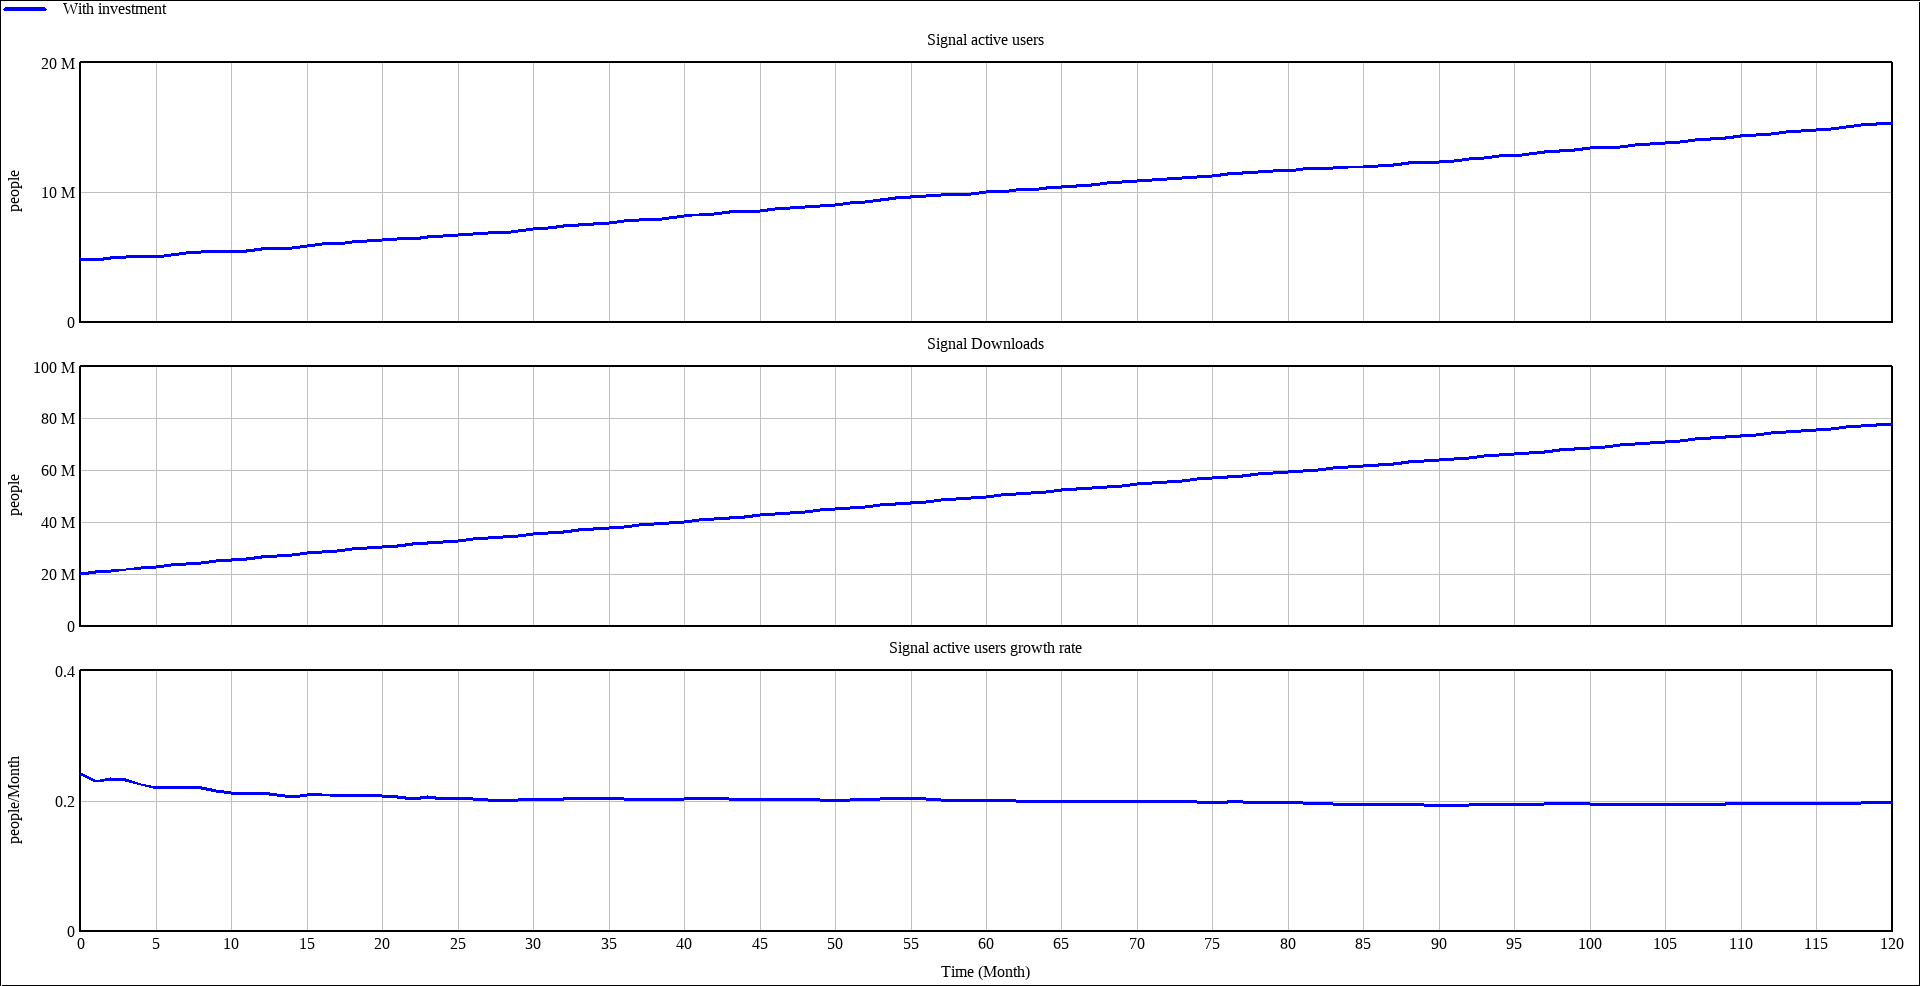
\includegraphics[width=17cm]{img/pessimist_model_signal.png}
       \caption{Resultados do crescimento do número de utilizadores ativos, do número de \textit{downloads} e do valor da relação entre o número de \textit{downloads} e o número de utilizadores ativos do \textit{Signal}, obtidos numa execução pessimista.}
       \label{model:pessimist_signal_model}
   \end{center}
\end{figure}

Como seria expectável, as duas aplicações concorrentes apresentaram um crescimento muito superior ao do modelo neutro, como se pode verificar nos gráficos da figura \ref{model:pessimist_others_model}.

\begin{figure}[H]
   \begin{center}
       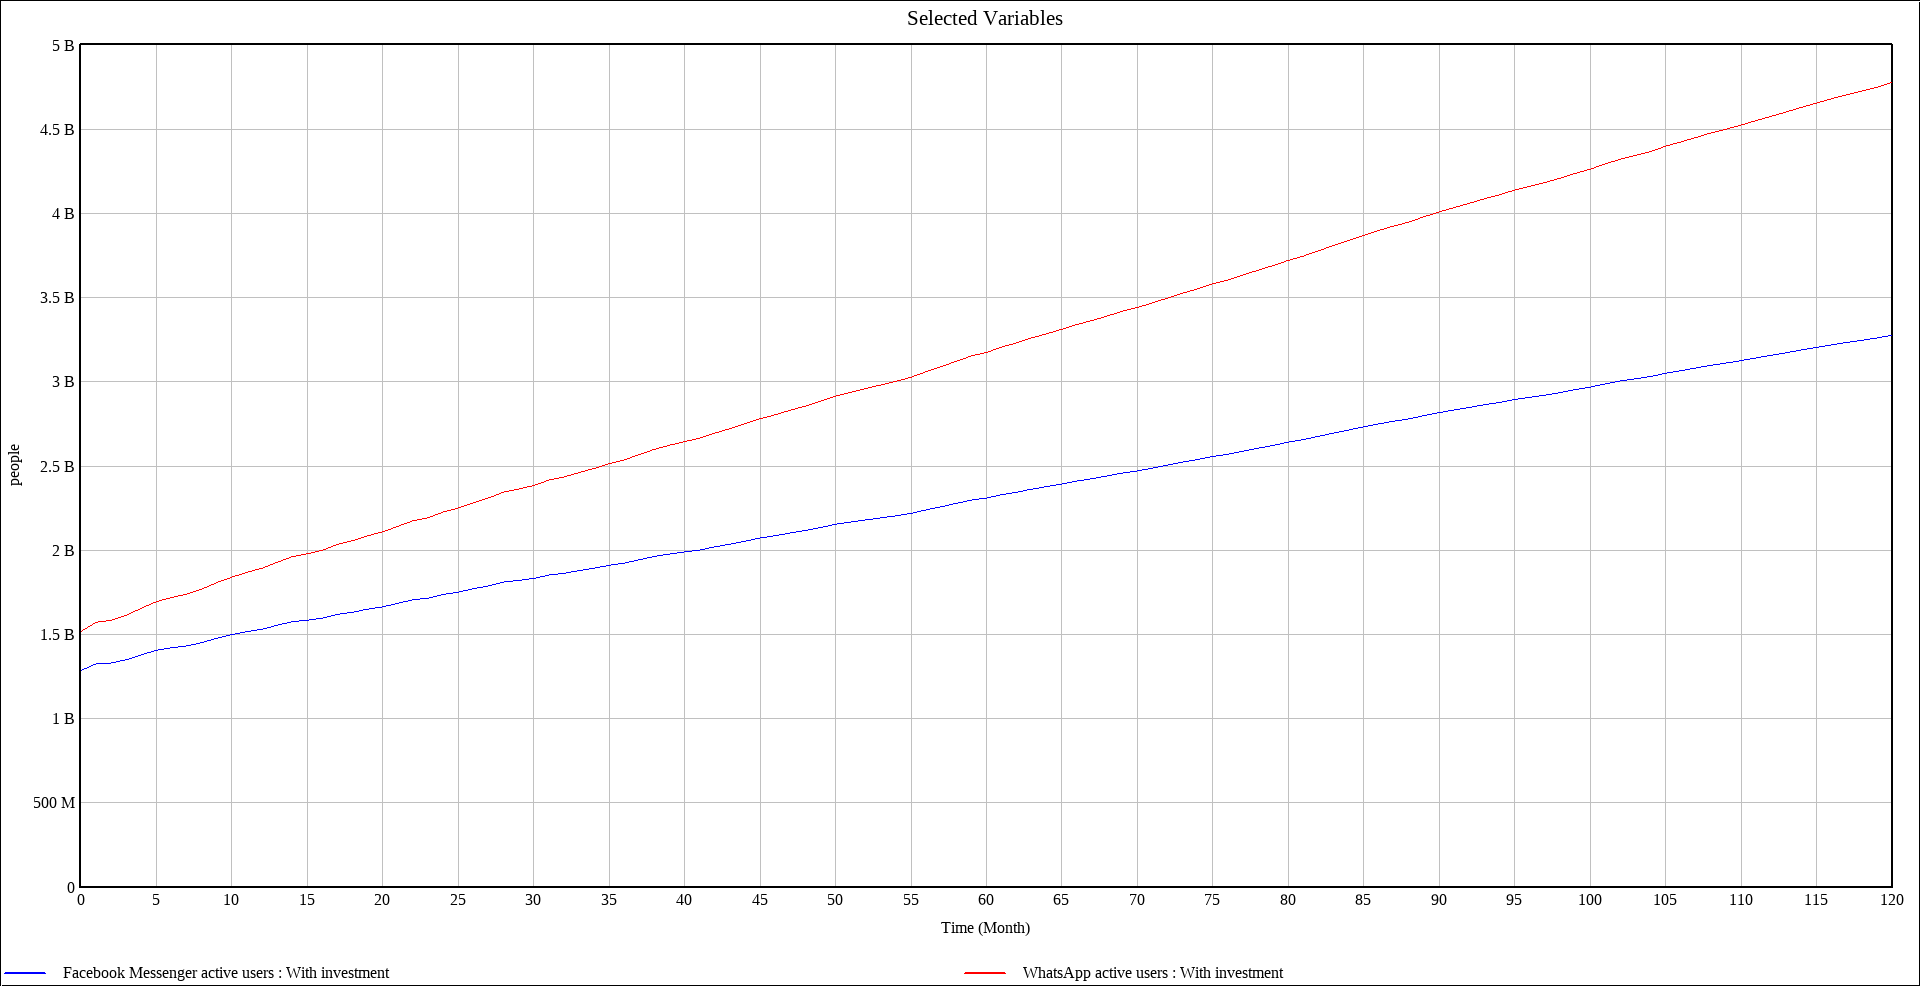
\includegraphics[width=17cm]{img/pessimist_model_others.png}
       \caption{Resultados do crescimento do número de utilizadores ativos das aplicações concorrentes, obtidos numa execução pessimista.}
       \label{model:pessimist_others_model}
   \end{center}
\end{figure}


\subsection{Modelo otimista}

Num modelo otimista foi alterada a probabilidade de ocorrerem investimentos (agora de $\frac{1}{12}$) e estes possuem agora um valor máximo superior (de 100 milhões de dólares). Para além disso, tendo em conta o maior número de investimentos, foram aumentados também os valores máximo e mínimo dos gastos mensais do \textit{Signal}, passando a ser de 1.5 e 0.7 milhões de dólares, respetivamente. Os resultados do crescimento do \textit{Signal} estão apresentados nos gráficos da figura \ref{model:optimistic_signal_model}. Como é percetível, são valores muito diferentes e superiores aos valores analisados até aqui, sendo que o número de utilizadores ativos alcança valores superiores a 40 milhões de utilizadores.

\begin{figure}[H]
   \begin{center}
       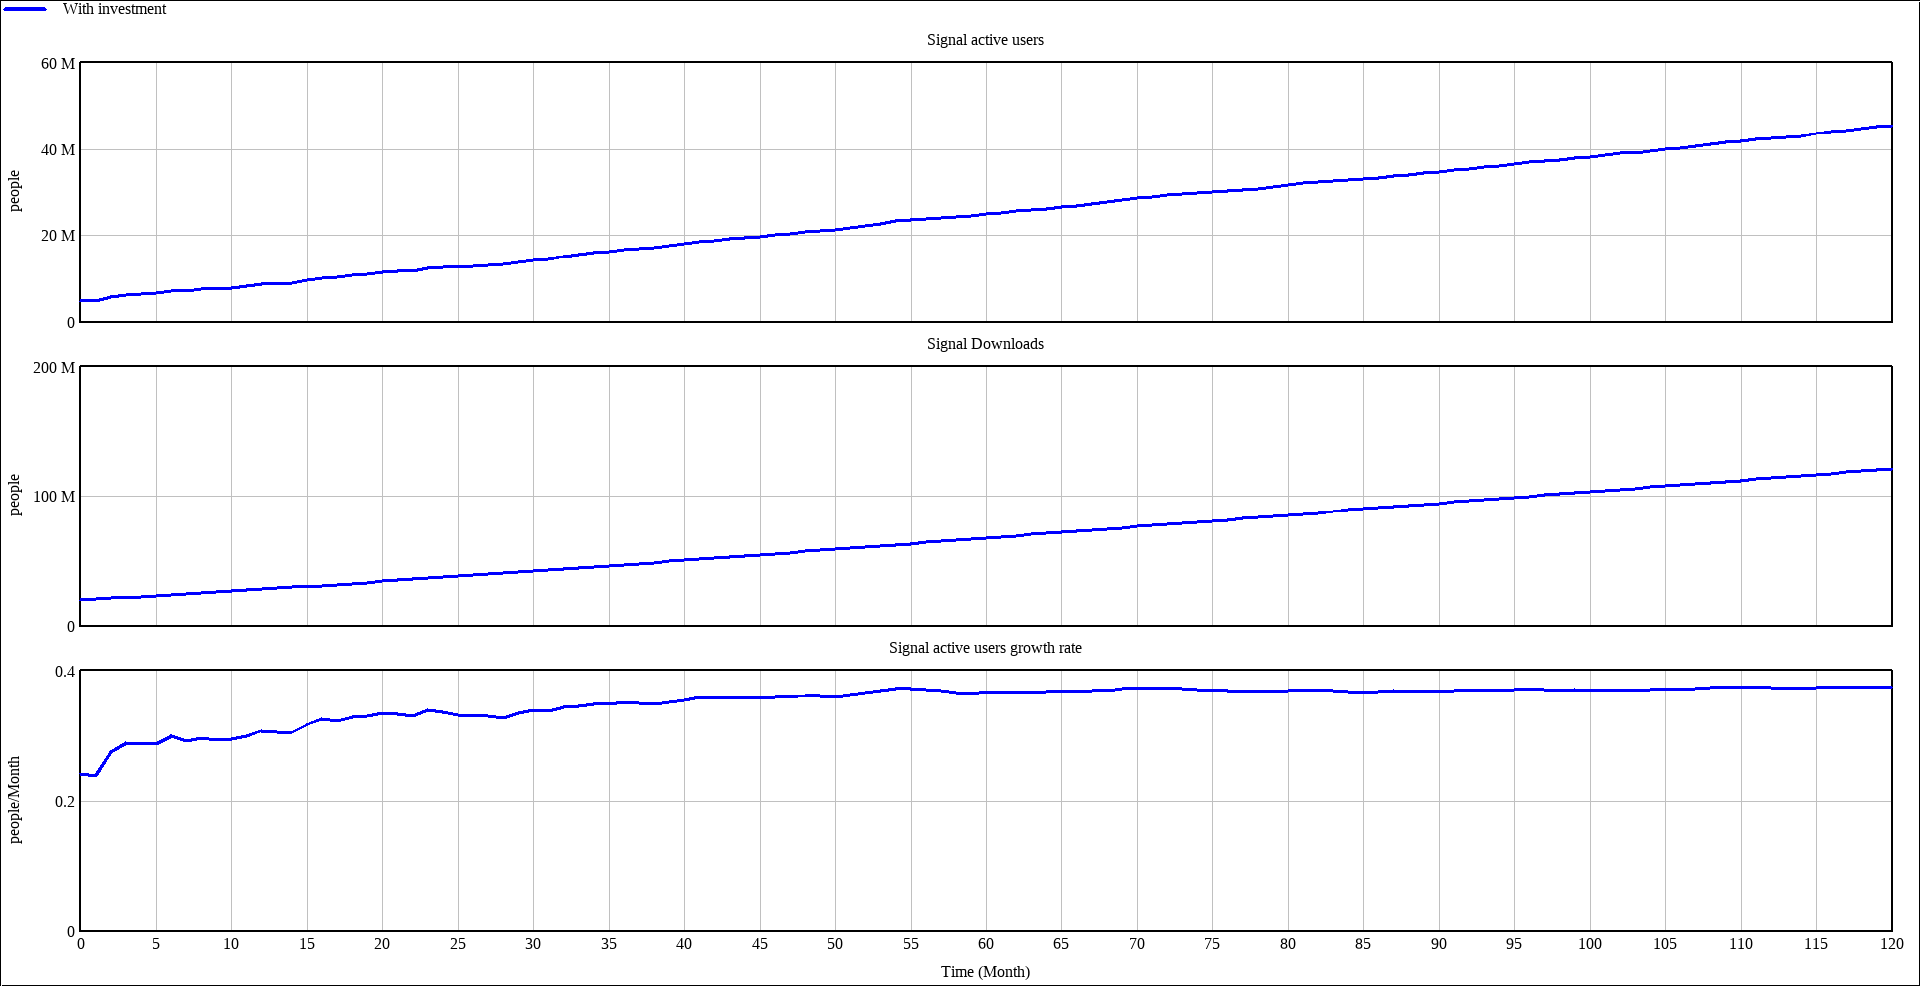
\includegraphics[width=17cm]{img/optimistic_model_signal.png}
       \caption{Resultados do crescimento do número de utilizadores ativos, do número de \textit{downloads} e do valor da relação entre o número de \textit{downloads} e o número de utilizadores ativos do \textit{Signal}, obtidos numa execução otimista.}
       \label{model:optimistic_signal_model}
   \end{center}
\end{figure}

Já as aplicações concorrentes, possuem um aumento do número de utilizadores ativos muito inferiores aos verificados nas execuções passadas, como é verificável nos gráficos da figura \ref{model:optimist_others_model}.

\begin{figure}[H]
   \begin{center}
       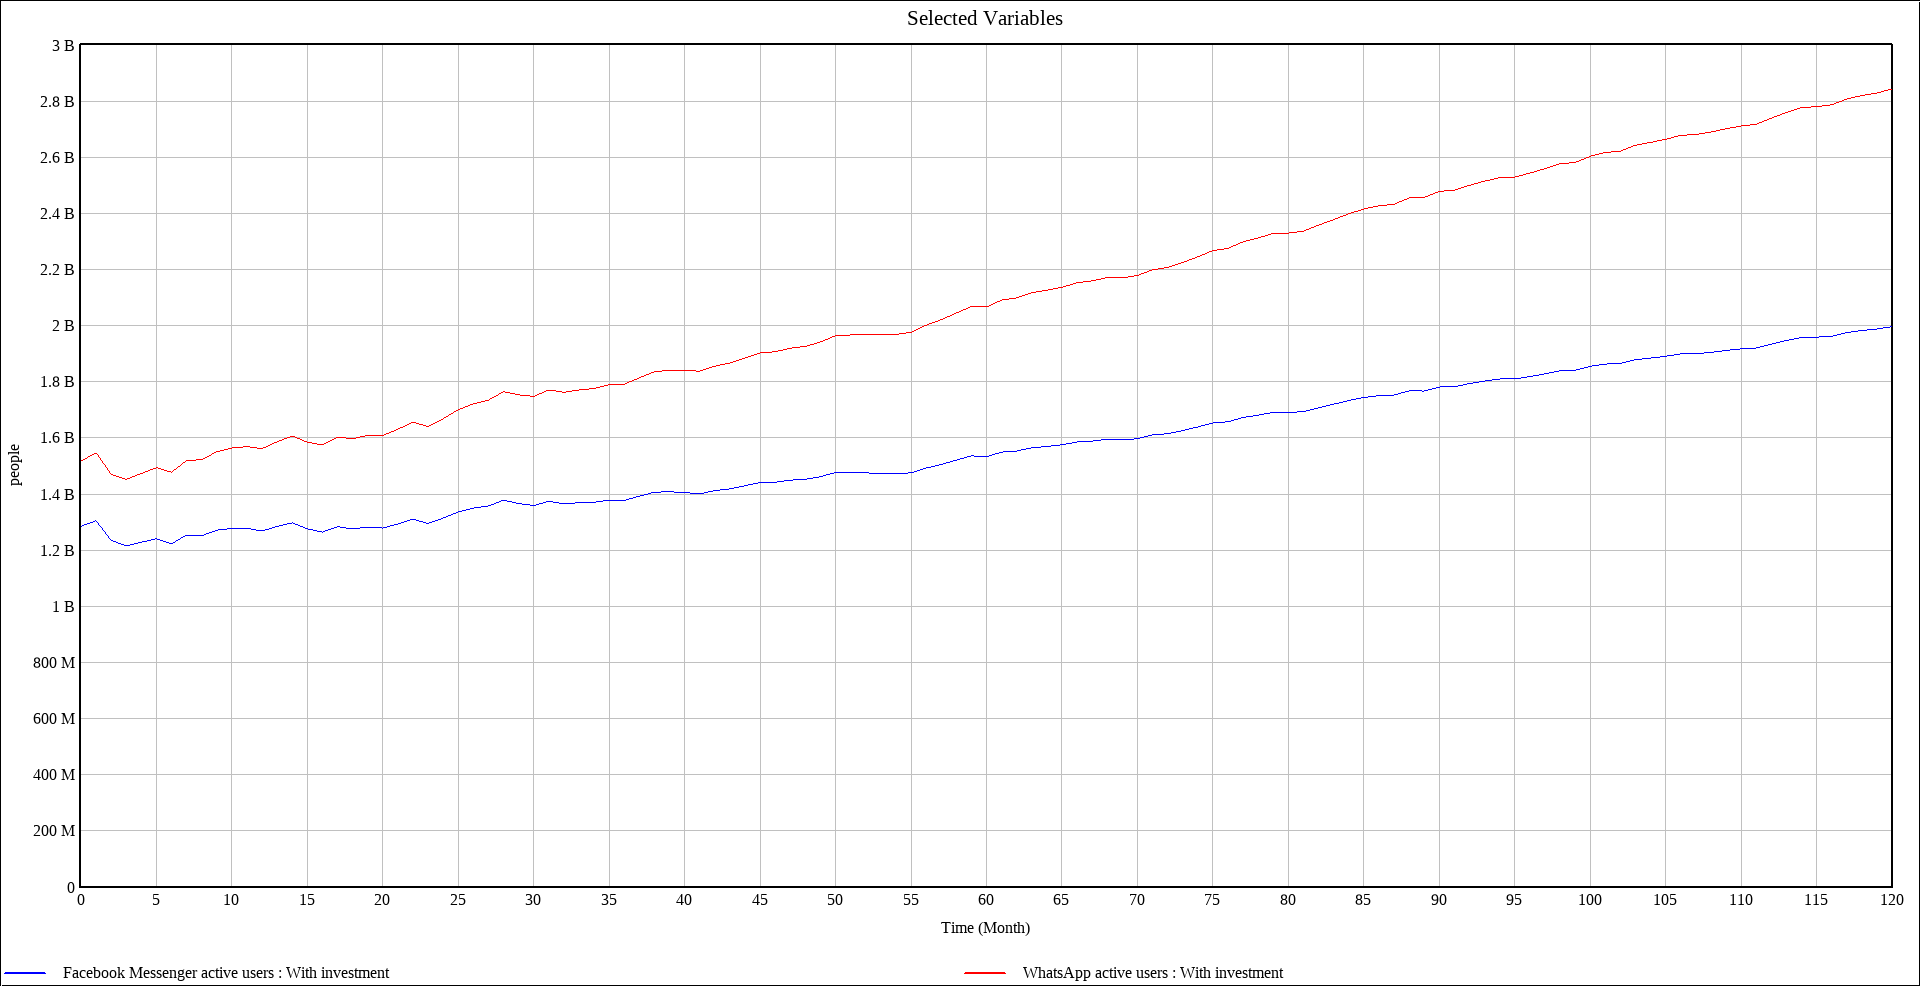
\includegraphics[width=17cm]{img/optimist_model_others.png}
       \caption{Resultados do crescimento do número de utilizadores ativos das aplicações concorrentes, obtidos numa execução otimista.}
       \label{model:optimist_others_model}
   \end{center}
\end{figure}
